\chapter{光学系の構成部品}
本研究ではコリメータ及び結像器にアクロマティックレンズ,検出器にはCCDカメラを用いる.

\section{アクロマティックレンズ}
アクロマティックレンズとは異なる二つのレンズが組み合わされたレンズである.
一般に低屈折率ガラスを用いたの正レンズと高屈折率のガラスを用いた負レンズで構成されている.

アクロマティックレンズの特徴として色収差が補正されているという点がある.
色収差とはガラスの屈折率が波長によって変化することから生まれる焦点距離のずれのことである.
アクロマティックレンズでは構成する二つのレンズが補完しあうことにより,単レンズと比べて色収差を抑えることができる.
Fig.\ \ref{fig:achromaticlense}でアクロマティックレンズが色収差を抑えていることを示す.
\begin{figure}[htbp]
    \centering
    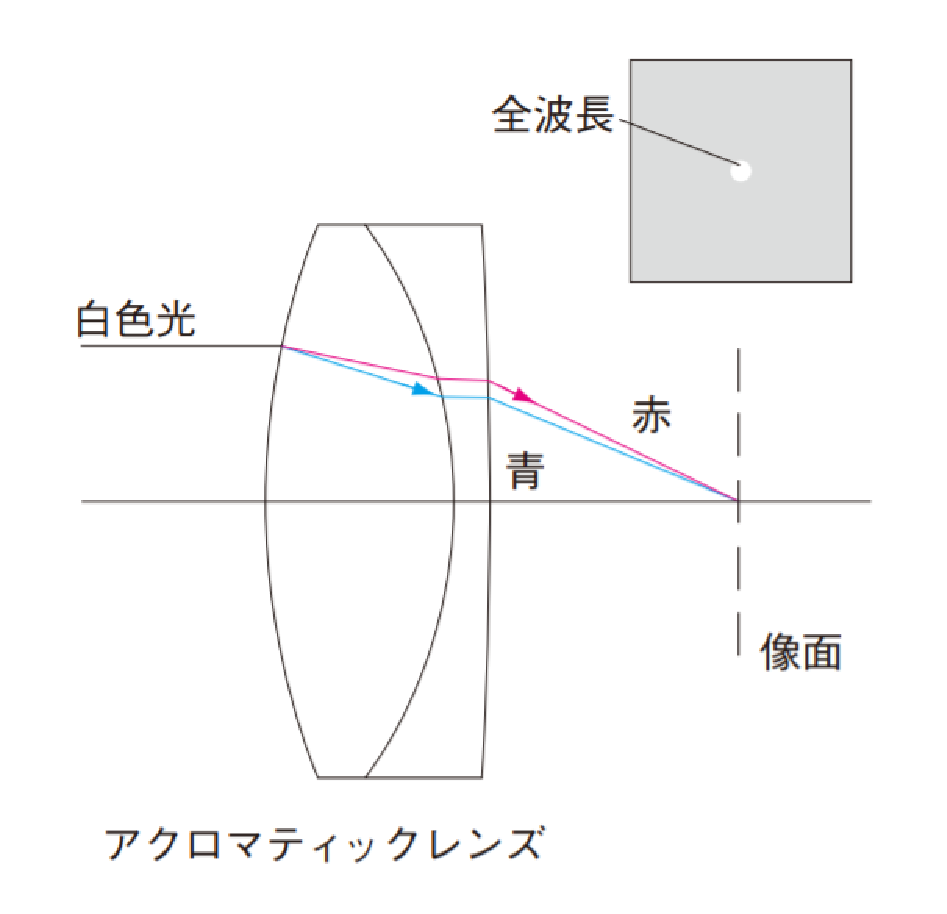
\includegraphics[scale=0.6]{figure/achromaticlense.pdf}
    \caption{アクロマティックレンズでの色収差の補正\cite{achromatic_lens}}
    \label{fig:achromaticlense}
\end{figure}
また,同様に色収差のみでなく球面収差も改善されており,レンズの有効径が大きい場合でも単レンズと比べて小さなスポット径を得ることができる.



% ここで,osloを用いてこのアクロマティックレンズがどのぐらいのスポット径に集光されるのかシミュレーションを行った.



% http://www.mekatoro.net/digianaecatalog/chuo-sougou/book/chuo-sougou-P0904.pdf

